\begin{abstract*}
\section{Introductie}
\label{cha:D:intro}
\subsection{De nood aan data integratie methoden}
Recente technologische vooruitgang zorgt ervoor dat datasets groter en groter worden. Dit is een trend die in vele gebieden merkbaar is, ook in het biomedische veld. Met grotere datasets bedoelen we dat de datasets zowel in aantal variabelen toenemen, als in het aantal datapunten. Het toenemende aantal variabelen is vooral te wijten aan de technologie. We zijn op het punt gekomen dat we relatief goedkoop ieders DNA kunnen uitlezen. Als we dan weten dat een gemiddelde persoon zo'n 20.000 tot 25.000 genen heeft die coderen voor prote\"inen, dan is het niet moeilijk om je in te beelden dat datasets duizenden variabelen bevatten. Een ander voorbeeld vinden we in de vooruitgang van beeldvormingsinstrumenten. Elk ziekenhuis beschikt tegenwoordig over talloze gigantisch geavanceerde scanners (MRI, PET, ...) die uiterst nauwkeurige afbeeldingen kunnen maken. Uit deze afbeeldingen kunnen heel wat variabelen worden afgeleid. Dit zijn slechts twee voorbeelden die aantonen dat het aantal variabelen enorm groeit. Naast deze groei zien we ook dat het aantal datapunten in de datasets stijgt. Ook dit heeft meerdere oorzaken. Een eerste oorzaak is simpelweg het feit dat we nu meer gegevens kunnen opslaan dan vroeger. Het is niet langer ongewoon om gigabytes of zelfs petabytes aan gegevens bij te houden. Een tweede oorzaak is dat onderzoekers over heel de wereld ijveren tot openstelling van gegevens. Als alle onderzoekers hun gegevens publiek delen met de hele wereld, dan heeft iedereen gewoonweg meer datapunten om te analyzeren, wat uiteindelijk de algemene vooruitgang zou stimuleren. \\ \\
De groei van datasets brengt echter ook problemen met zich mee, we moeten namelijk zoeken naar technieken om al deze gegevens van verschillende bronnen op de beste manier met elkaar te combineren tot een coherent systeem.

\subsection{Doel en werkwijze}
Het doel van dit thesis is om enkele integratie strategie\"en te ontwikkelen en aan te tonen dat deze strategie\"en een impact hebben op de performantie van predictieve modellen. In plaats van predictieve modellen te bouwen voor individuele datasets zullen we dus proberen om meerdere datasets te combineren en 1 predictief model te bouwen dat alle gegevens gebruikt en dat een betere performantie biedt dan alle andere individuele modellen. Om dit te doen is het belangrijk dat we eerst goed begrijpen wat een predictief model is en hoe we er een kunnen opbouwen. Het eerste hoofdstuk legt uit wat we bedoelen met predictieve modellen en stelt het eerste type voor: het logistieke regressie model. Het volgende hoofdstuk geeft een tweede type van predictief model dat we overlevingsmodellen noemen. Specifiek zullen we ons focussen op het cox model. Vervolgens zullen we de verschillende integratie strategie\"en voorstellen. Om aan te tonen dat deze strategie\"en effectief een impact hebben op de performantie van de modellen zullen we twee concrete case-studies tonen. De eerste case-studie zal logistieke regressie gebruiken om predictieve modellen te bouwen, gebruik makend van alle integratie strategie\"en. De tweede case-studie zal hetzelfde doen voor de survival modellen. In beide case-studies zullen alle modellen ge\"evalueerd worden met geschikte technieken. \\ \\
Om het hele proces te ondersteunen hebben we een interactieve applicatie ontwikkeld die in staat is om de performantie van predictieve modellen te evalueren. Dit liet ons toe om de twee case-studies op te bouwen, maar het vormt ook een platform voor toekomstig onderzoek.

\section{Predictieve modellen}
\label{cha:D:predictieve-modellen}

\subsection{Introductie}
\label{sec:D:pm-introductie}
In dit hoofdstuk leggen we uit wat een predictief model inhoudt en hoe deze worden opgebouwd. We zullen hiervoor twee concrete voorbeelden gebruiken: logistieke regressie en cox survival modellen. Verder leggen we ook het concept van regularisatie uit, dit zal belangrijk blijken in het volgende hoofdstuk over integratie strategie\"en. Tenslotte zullen we ook kort uitleggen wat validatie inhoudt.

\subsection{Wat is een predictief model?}
\label{sec:D:pm}
Een predictief model is een relatie tussen input variabelen en een doelfunctie (doel variabele). De taak van een predictief model is om een waarde te voorspellen voor de doelfunctie, gegeven een set van waarden voor de input variabelen. Bijvoorbeeld: we kunnen een predictief model bouwen dat de relatie probeert voor te stellen tussen een datum en de gemiddelde temperatuur op die dag. De input is hier de datum, de doelfunctie (of output) is de gemiddelde temperatuur voor die dag. We kunnen ons inbeelden dat er tussen deze twee variabelen een verband bestaat. Een datum ergens in de zomer zal namelijk een relatief hoge gemiddelde temperatuur opleveren, en een dag in de winter een relatief lage temperatuur. We weten dit omdat we jarenlang ervaring hebben opgebouwd en ons hebben gerealizeerd dat het in de zomer normaal warm is en in de winter koud. Dit is precies wat we proberen te vatten met een predictief model, het onderliggende patroon. En de manier om daartoe te komen is door ervaring op te bouwen. Op eenzelfde manier gaan we proberen het model ervaring te laten opbouwen, we noemen dit dan 'het model trainen'. We gaan het model voorbeelden tonen van wat we willen dat het model leert, en het model zal hieruit leren en intern een representatie opbouwen om zijn kennis voor te stellen. In het eerder gegeven voorbeeld zouden we, om het model te trainen, een hele lijst met data en de corresponderende gemiddelde temperatuur voor die dag tonen aan het model, dit noemen we de training set. Het model zal dan intern een representatie opbouwen van zijn kennis en als alles goed verloopt zal deze representatie inderdaad weergeven dat het in de zomer normaal warmer is en in de winter normaal kouder. Welke representatie het model intern gebruikt is een keuze die we zelf maken, en hangt af van het type van patronen dat we willen representeren en dus van de relatie die we denken dat er bestaat tussen de input en de doelfunctie. Er zijn talloze representaties mogelijk, in dit thesis focussen we ons op lineaire representaties. Dit wil zeggen dat we veronderstellen dat we een lineaire combinatie kunnen maken van de input variabelen, en daarmee accuraat de doelfunctie kunnen benaderen. Afhankelijk van het type van de doelfunctie die we willen benaderen zijn hier echter nog verschillende methoden voor, in de volgende secties bekijken we twee concrete voorbeelden: logistieke regressie en cox modellen.

\subsection{Logistieke regressie}
\label{subsec:D:pm-logistieke-regressie}
In logistieke regressie maken we twee veronderstellingen. De eerste is dat er een lineair verband bestaat tussen de input variabelen en de doelfunctie. De tweede is dat, in de training set, de waarden van de doelfunctie het resultaat zijn van een binomiaalverdeling. Denk hierbij bijvoorbeeld aan het genezen of niet-genezen van een kankerpati\"ent, in onze training set zullen we enkel de waarden 'genezen' en 'niet-genezen' aantreffen, maar we weten dat onderliggend deze waarden gegenereerd zijn met een bepaalde probabiliteit van overleving. De taak in logistieke regressie (en dus van ons predictief model) is om deze onderliggende probabiliteit te schatten. Stel dat we N voorbeeld datapunten hebben waarbij elk datapunt M input variabelen bevat, dan kunnen we logistieke regressie als volgt neerschrijven:
\begin{equation}
\begin{split}
\hat{y}_{n} = \theta(\sum_{i=1}^{M}w_{i}x_{in})= \theta(\bm{w^{T}x_{n}}) \qquad for\ n=1..N
\end{split}
\end{equation}
hierin is
\begin{itemize}
	\item $\hat{y}_{n}$ is de geschatte waarde voor de probabiliteit voor datapunt $n$
	\item $w_{i}$ is de model parameter (co\"effici\"ent) voor input variabele $i$
	\item $x_{in}$ is de waarde voor input variabele $i$ voor datapunt $n$
	\item $\bm{w^{T}x}$ is de vector notatie voor het inwendig product van $\bm{w}$ en $\bm{x}$
	\item $\theta(x)$ is de logistieke functie. Een voorbeeld voor deze function is $\frac{e^{x}}{1+e^{x}}$
\end{itemize}
Deze formule geeft weer dat, gegeven een input vector $\bm{x_{n}}$, ons model in staat is om zijn interne kennis (met representatie $\bm{w}$) te gebruiken om een waarde te voorspellen ($\hat{y}_{n}$) voor de probabiliteit. De functie $\theta$ is de logistieke functie, deze functie is een mapping van de re\"ele getallen naar het bereik $[0..1]$ en zorgt ervoor dat we het resultaat kunnen interpreteren als een probabiliteit.

\subsection{Cox proportionele risico modellen}
Het volgende type modellen dat we bespreken valt onder de noemer van survival (overlevings-) modellen. Bij deze modellen proberen we de de tijd te schatten tot het voorkomen van een bepaald event op basis van de input variabelen. In ons geval is het event dat we bestuderen het overlijden van patienten aan kanker, vanaf nu zullen we dit ook zo behandelen. De doelfunctie wordt daarom ook wel de overlevingsfunctie genoemd. Om overlevingsfuncties te plotten worden vaak kaplan-meier curves gebruikt, op figuur \ref{fig:D:cox-example-kaplan-meier} worden twee voorbeeld overlevingsfuncties getoond.	
\begin{figure}
	\centering
	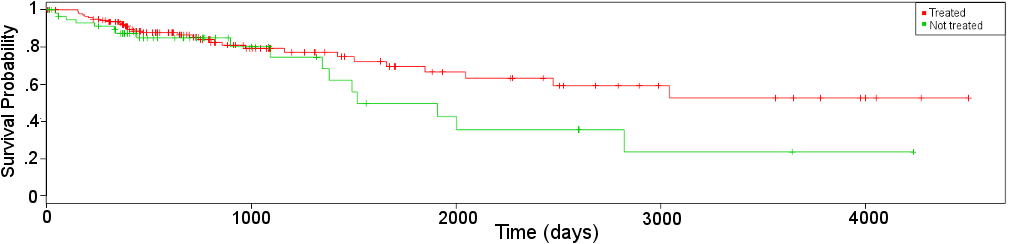
\includegraphics[scale=0.4]{images/example_kaplan_meier_curve}
	\caption{Voorbeeld kaplan-meier survival curves. De X-as geeft de tijd weer, de Y-as geeft de kans weer op overleving.}
	\label{fig:D:cox-example-kaplan-meier}
\end{figure}
Bij overlevingsanalyze wordt echter ook vaak gebruik gemaakt van de zogenaamde hazard (of risico) functie. Deze functie geeft weer wat het risico is dat op een gegeven tijdstip het event zich voordoet. In het cox proportionele risico model dat we zullen gebruiken wordt deze risico functie als volgt genoteerd:
\begin{equation}
\begin{split}
\lambda_{i}(t) = \lambda_{0}(t)e^{X_{i1}\beta_{1} + ... + X_{iN}\beta_{N}}
\end{split}
\end{equation}
where
\begin{itemize}
	\item $\lambda_{i}(t)$ is het risico op overlijden voor pati\"ent i op tijdstip t.
	\item $\lambda_{0}(t)$ is de baseline risico op tijdstip t, dit is het risico op overlijden zonder enige invloed van de input variabelen.
	\item $X_{i1} ... X_{iN}$ zijn de waarden voor de input variabelen voor pati\"ent i.
	\item $\beta_{1} ... \beta_{N}$ zijn de waarden voor de parameters van het model (de kennis representatie).
\end{itemize}
Een tweede interessant concept is wat met noemt de risico-verhouding (hazard ratio). Dit is de verhouding van twee risico functies:
\begin{equation}
\label{eq:D:cox-hazard-ratio}
\begin{split}
\frac{\lambda_{i}(t)}{\lambda_{j}(t)} 
= \frac{\lambda_{0}(t)e^{X_{i1}\beta_{1} + ... + X_{iN}\beta_{N}}}{\lambda_{0}(t)e^{X_{j1}\beta_{1} + ... + X_{jN}\beta_{N}}}
= e^{(X_{i1}-X_{j1})\beta_{1} + ... + (X_{iN}-X_{jN})\beta_{N}}
\end{split}
\end{equation}
Merk op dat de vorm van de risico functie een keuze is die we zelf hebben gemaakt, door te kiezen voor cox proportionele risico modellen. Deze keuze heeft twee heel belangrijke gevolgen die duidelijk worden in de formule van de risico-verhouding (\ref{eq:D:cox-hazard-ratio}). Het eerste gevolg is dat risico-verhoudingen onafhankelijk zijn van de tijd. Dit wil zeggen dat de risico-verhouding tussen twee pati\"nten dus niet verandert doorheen de tijd. Vandaar ook de naam 'proportionele risico modellen'. Het tweede gevolg is dat veranderingen in de input variabelen een multiplicatief effect hebben op het risico. Dit kunnen we ook zien in formule \ref{eq:D:cox-hazard-ratio}, maar is nog duidelijker als we de risico-verhouding neerschrijven met in de noemer het risico voor een pati\"ent met bepaalde waarden voor de input variabelen, en in de teller het risico voor een pati\"ent met exact dezelfde input waarden, behalve voor 1 variabele $X_{j}$ een verhoging met 1:
\begin{equation}
\begin{split}
\frac{\lambda(t|X_{j}+1)}{\lambda(t|X_{j})} = e^{(X_{j}+1-X_{j})\beta_{j}} = e^{\beta_{j}}
\end{split}
\end{equation}
We zien dus dat een verhoging met 1 voor een input variabele, het risico doet veranderen met $e^{\beta_{j}}$, de exponenti\"ele van de bijhorende co\"effici\"ent.

\subsubsection{Het predictief overlevingsmodel}
Net zoals bij logistieke regressie hebben we hier dus te maken met een set gewichten die onze kennis representatie voorstellen. We zullen ook heel analoog een iteratief algoritme gebruiken om deze gewichten te bepalen. We zullen het model een hele reeks voorbeeld datapunten tonen (input variabelen met bijhorende overlevingskans) om zo het model ervaring te laten opbouwen en op die manier zo goed mogelijk de overlevingskansen van pati\"enten te laten schatten.

\subsection{Regularizatie}
Een belangrijk concept dat we moeten toevoegen aan onze modellen is regularizatie. Herinner je uit sectie \ref{sec:D:pm} dat we een predictief model opbouwen door het een reeks voorbeeld datapunten te geven om het op die manier zijn interne representatie van de kennis te laten opbouwen. In beide voorbeeld modellen die we hebben gezien is deze representatie en set van gewichten. Het concept van regularizatie houdt in dat we een of meerdere beperkingen gaan opleggen aan deze gewichten. Het doel hiervan is om bepaalde modellen (bepaalde combinaties van gewichten) te prefereren boven anderen. De onderliggende gedachte is dat we gaan trachten van simpele modellen te bekomen, die een vloeiende functie voorstellen. We doen dit om te voorkomen dat het model patronen gaat vinden die er eigenlijk niet zijn of die enkel het resultaat zijn van ruis is de gegevens. Er zijn verschillende beperkingen mogelijk die we kunnen opleggen, en elk krijgen ze hun eigen naam: de ridge penalty, de lasso penalty en het elastisch-net pentalty.
\subsubsection{Ridge penalty}
Bij de ridge penalty (ook wel $L_{2}$ panalty genoemd) is de beperking die we opleggen de volgende:
$$
\sum_{i=1}^{N}w_{i}^{2} \leq C
$$
Deze beperking zal ervoor zorgen dat gewichten klein worden gehouden, en het dus onmogelijk wordt dat een gewicht extreem groot wordt relatief ten opzichte van de andere gewichten.
\subsubsection{Lasso penalty}
Bij de lasso penalty (ook wel $L_{1}$ penalty genoemd) is de beperking:
$$
\sum_{i=1}^{N}\lvert w_{i}\rvert \leq C
$$
Deze beperking heeft ook als gevolg dat de gewichten klein worden gehouden, maar heeft als extra dat gewichten ook effectief 0 worden indien ze niet belangrijk genoeg zijn in het model. We noemen dit daarom ook 'variabele selectie'. Gebruik van de lasso penalty heeft als gevolg dat het resulterende model vaak minder parameters gebruikt, omdat het enkel deze parameters gebruikt die echt belangrijk zijn. Deze techniek zal zeer belangrijk blijken bij een van de integratie technieken die later worden besproken.
\subsubsection{Elastisch-net penalty}
Bij het elastisch-net penalty is de beperking een combinatie van de ridge en lasso penalties:
$$
\alpha \sum_{i=1}^{N}w_{i}^{2} + (1-\alpha)\sum_{i=1}^{N}\lvert w_{i}\rvert \leq C
$$
Deze methode heeft daarom ook eigenschappen van zowel ridge als lasso, en met de parameter $\alpha$ kan men kiezen hoezeer men wil aanleunen bij een van de twee technieken. Dit vormt als het ware een gulden middenweg.
\subsubsection{De parameter $\lambda$}
Wanneer met regularizatie echter toepast op een concreet model, zal men altijd het optimalisatie probleem met beperking proberen omvormen naar een equivalent optimalisatie probleem zonder beperking. Bij deze omvorming introduceert men dan meestal een parameter $\lambda$ die als vervanging dient voor de parameter $C$ in bovenstaande beperkingen. $\lambda$ kan men zien als de hoeveelheid regularizatie die men wil gebruiken. Hoe groter $\lambda$ hoe sterker de beperking en dus hoe kleiner $C$. Hoe kleiner $\lambda$, hoe minder regularizatie, hoe groter $C$.

\subsection{Validatie}
Het laatste concept dat we moeten behandelen is validatie. Dit zal ons toelaten om een getraind model te evalueren. Bij validatie delen we onze dataset op in twee delen: een training set en een validatie set. De training set kennen we reeds, deze datapunten zullen we gebruiken om een model te trainen. Merk op dat we nu echter nog datapunten over hebben die niet gebruikt werden voor de training, dit is de validatie set. We zullen het getrainde model vragen om voor deze datapunten een predictie te berekenen voor de output variabelen. We kennen van de datapunten in de validatie set echter de correcte output waarde. We kunnen vervolgens dus de output van ons predictief model vergelijken met de juiste waarde, en op die manier een idee krijgen hoe goed ons predictief model presteert. \\ \\
Merk echter op dat de training set die we gebruiken om het model te trainen kleiner is dan de volledige dataset waarover we beschikken. We houden inderdaad de datapunten in de validatie set opzij. We willen echter zoveel mogelijk datapunten gebruiken om te trainen, want dan bekomen we een beter model. Langs de andere kant willen we ook genoeg datapunten in de validatie set om een goed beeld te krijgen van de performantie van het bekomen model. Een oplossing voor deze contradictie is cross-validatie. Bij cross-validatie delen we onze dataset op in K (vaak 10) gelijke stukken. We gebruiken 1 van de K stukken als validatie set, en de andere K-1 stukken als training set. We herhalen dit proces K keren, waarbij we iedere keer een ander stuk nemen als validatie set. Op die manier hebben we op het einde voor elk datapunt in onze dataset een predictie. Deze predicties kunnen we dan vergelijken met de echte waarden en dit zal ons een redelijk goed beeld geven van de performantie van het model dat we zouden bekomen indien we op de volledige dataset zouden trainen.

\section{Integratie technieken}
\label{cha:D:integratie}

\subsection{Inleiding}
\label{sec:D:integratie-inleiding}
In dit hoofdstuk stellen we drie verschillende integratie technieken voor. Eerst zullen we kort overlopen hoe de data eruit ziet waar we van vertrekken, en vervolgens zullen we de drie technieken overlopen. De eerste strategie noemen we vroege-integratie en is gebaseerd op het aan elkaar voegen van datasets. De tweede strategie heet late-integratie en is gebaseerd op het concept van 'ensemble-learning'. De laatste techniek heet parti\"ele integratie en maakt gebruik van de variabele selectie in de lasso regularizatie. 

\subsection{Beschrijving van de data}
\label{sec:D:integratie-beschrijving}
Integratie duidt op het combineren van verschillende elementen. In dit geval zijn de elementen waarmee we te maken hebben datasets. Herinner je dat we, om een model te trainen, een lijst van gelabelde datapunten nodig hadden. Zo een lijst noemen we een dataset. Nu hebben we te maken met meerdere datasets, en moeten we een strategie bedenken om deze verschillende datasets te gebruiken om een model te trainen. Merk op dat het noodzakelijk is om datapunten over verschillende datasets aan elkaar te koppelen. Met andere woorden, alle datapunten in de datasets moeten een vorm van unieke identificatie krijgen waardoor we gegevens van verschillende datasets, die spreken over eenzelfde datapunt, aan elkaar kunnen koppelen.

\subsection{Vroege integratie}
\label{sec:D:integratie-vroeg}
Bij vroege integratie gaan we op voorhand (voor het trainen) alle gegevens over eenzelfde datapunt aan elkaar koppelen. Dit is mogelijk omdat elk datapunt een unieke identificatie krijgt. We kunnen dit bezien als het aan elkaar plakken van alle datasets, waardoor we uiteindelijk overblijven met slechts $\acute{e}\acute{e}n$ grotere dataset. Een schematisch overzicht van vroege integratie wordt gegeven op figuur \ref{fig:D:integratie-vroeg}.
\begin{figure}
	\centering
	\includegraphics[scale=.8]{images/early_integration}
	\caption{Schema voor vroege integratie}
	\label{fig:D:integratie-vroeg}
\end{figure}

\subsection{Late integratie}
\label{sec:D:integratie-laat}
Bij late integratie zullen we eerst voor elke dataset apart een model trainen. Als het aantal datasets gelijk is aan $D$ dan zullen we dus ook $D$ predictieve modellen bekomen. Wanneer we dan voor een nieuw (ongezien) datapunt een predictie moeten maken, zullen we dit datapunt aan elk van de $D$ predictieve modellen geven. Zij zullen elk individueel een predictie maken. Vervolgens combineren we de $D$ voorspelde waarden in een lineaire combinatie om tot een finale predictie waarde te komen. Indien we geen extra waarde willen hechten aan een van de $D$ modellen kunnen we voor deze lineaire combinatie gewoon het gemiddelde nemen van alle voorspelde waarden. \\ \\
In het veld van machine-leren is het concept van ensemble-leren reeds bekend. Dit houdt in dat voor een bepaald probleem meerdere verschillende modellen worden getraind op dezelfde dataset. Het combineren van de output van de verschillende modellen kan dan een beter resultaat geven vergeleken met een enkel model. Dit komt doordat de verschillende modellen mogelijks fouten maken op verschillende vlakken, en door uitmiddeling van de outputs worden deze fouten relatief verkleint. De late integratie techniek neemt deze gedachtengang over. We gebruiken nu niet meerdere modellen voor dezelfde dataset, maar we gebruiken meerdere modellen voor meerdere datasets. Door deze uitmiddeling hopen we echter eenzelfde foutenreductie te bekomen. Een schematisch overzicht van de late integratie techniek wordt getoond op figuur \ref{fig:D:integratie-laat}.
\begin{figure}
	\centering
	\includegraphics[scale=.8]{images/late_integration}
	\caption{Schema voor late integratie}
	\label{fig:D:integratie-laat}
\end{figure}

\subsection{Parti\"ele integratie}
\label{sec:D:integratie-partieel}
De laatste methode die we voorstellen is de parti\"ele integratie. Deze methode vertrekt analoog aan de late integratie door voor elke dataset individueel een predictief model op te stellen. Belangrijk hierbij is op te merken dat bij het trainen van deze modellen de lasso regularizatie wordt gebruikt. Dit doen we om gebruik te maken van de variabele selectie eigenschap. Door deze variabele selectie zullen de resulterende modellen ons namelijk vertellen welke variabelen zij belangrijk achten in de datasets. De volgende stap is dan om uit elke dataset enkel die variabelen te extraheren die door de modellen geselecteerd werden. Deze geselecteerde gegevens worden dan aan elkaar geplakt zoals in de vroege integratie, op basis van unieke identificatie van de datapunten. Dit geeft ons een nieuwe, gereduceerde, dataset. Deze dataset gebruiken we vervolgens om opnieuw een predictief model op te stellen, dit is het finale ge\"integreerde model dat we zullen gebruiken voor predictie. Merk op dat deze techniek dus in twee stappen werkt, er zijn twee training fases. Een schematische voorstelling van de parti\"ele integratie wordt gegeven op figuur \ref{fig:D:integratie-partieel}.

\begin{figure}
	\centering
	\includegraphics[scale=.8]{images/intermediate_integration}
	\caption{Schema voor parti\"ele integratie}
	\label{fig:D:integratie-partieel}
\end{figure}

\section{Evaluatie van integratie methoden}
\label{cha:D:evaluatie}

\subsection{Introductie}
\label{sec:D:evaluatie-introductie}
In dit hoofdstuk zullen we onderzoeken of de verschillende integratie strategie\"en en impact hebben op de performantie van de resulterende modellen. We doen dit door in twee concrete case studies, op echte kankergegevens, een model uit te werken gebruikmakend van elke strategie. En vervolgens de bekomen modellen te evalueren met een passende metriek.

\subsection{Case studie 1: logistieke regressie}
\subsubsection{Case overzicht}
In de eerste case studie zullen we logistieke regressie modellen gebruiken. De gebruikte datasets komen van het Universitair Ziekenhuis te Leuven en betreffen gegevens van pati\"enten met darmkanker. Van deze pati\"enten zijn tijdens de behandeling scans genomen met een MRI scanner, PET scanner en DWI scanner. We hebben in dit geval dus te maken met drie datasets. De output variabele die we zullen trachten te voorspellen is een binaire versie van het pathologisch stadium van elke pati\"ent (zie appendix \ref{app:cancer-staging}). We kunnen stellen dat pati\"enten met een label 1 van de kanker zijn genezen, en pati\"enten met een label 0 niet. Deze output die het predictief model ons zal geven is dus een kans op genezing.
\subsubsection{Evaluatie methode}
We zullen de logistieke modellen evalueren met een Receiver-Operator Characteristic analyse. Herinner je dat we via cross-validatie voor elk datapunt in onze dataset een predictie konden bekomen. In het geval van logistieke regressie is deze predictie een probabiliteit. De output voor de datapunten in onze dataset zijn echter binaire waarden (de realisaties van de binomiaalverdeling). Om de twee te kunnen vergelijken moeten we een drempelwaarde defini\"eren. Als de voorspelde probabiliteit hoger is dan deze drempelwaarde dan voorspellen we een positieve output, anders een negatieve output. Voor elk datapunt zijn er hierbij dan vier scenario's mogelijk:
\begin{itemize}
	\item True Positive (TP): het model voorspelt een positieve output, en dat is correct
	\item True Negative (TN): het model voorspelt een negatieve output, en dat is correct
	\item False Positive(FP): het model voorspelt een positieve output, en dat is fout (type 1 fout)
	\item False Negative (FN): het model voorspelt een negatieve output, en dat is fout (type 2 fout)
\end{itemize}
Merk op dat we in dit geval niet enkel zeggen of het model juist of fout was, maar ook de type fout registreren. Dit laat ons toe om volgende begrippen van sensitiviteit en specificiteit te defini\"eren:
$$
sensitiviteit = \frac{\sum{TP}}{\sum{P}}
$$
$$
specificiteit = \frac{\sum{TN}}{\sum{N}}
$$
hierin zijn
\begin{itemize}
	\item $\sum{TP}$ het totale aantal true positives
	\item $\sum{P}$ is het totale aantal datapunten met positieve output in de dataset
	\item $\sum{TN}$ het totale aantal true negatives
	\item $\sum{N}$ is het totale aantal datapunten met negatieve output in de dataset
\end{itemize}
Het perfecte model, dat altijd juist voorspelt, heeft een sensitiviteit en specificiteit gelijk aan 1. In een realistische setting is dit echter zelden haalbaar. We willen beide metrieken echter zo dicht mogelijk bij 1. We kunnen nu een plot maken waarbij we op de sensitiviteit plotten in functie van de specificiteit voor verschillende waarden van de drempelwaarde. Merk op dat inderdaad verschillende drempelwaarden ervoor zullen zorgen dat het model verschillende voorspellingen maakt en dus sensitiviteit en specificiteit zullen be\"invloeden. De curve die we bekomen op deze plot noemt men een Receiver Operating Characteristic curve. Een voorbeeld curve wordt getoont op figuur \ref{fig:D:evaluation-roc}. De metriek die we zullen gebruiken is de oppervlakte onder deze ROC curve, ook wel afgekort AUC(Area Under the ROC Curve). Hoe hoger deze waarde, hoe groter de waarden voor sensitiviteit en specificiteit bij verschillende drempelwaarden, en dus hoe beter ons predictief model.
\begin{figure}
	\centering
	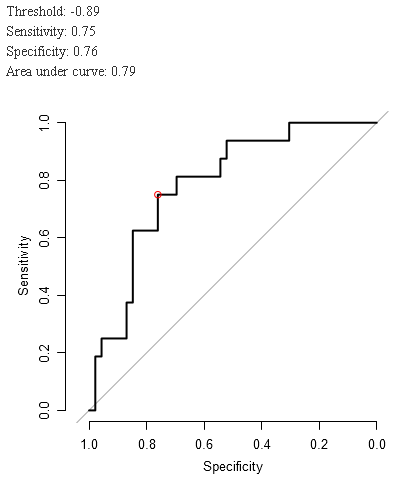
\includegraphics[scale=.7]{images/roc_curve}
	\caption{Voorbeeld ROC curve en metrieken}
	\label{fig:D:evaluation-roc}
\end{figure}

\subsection{Resultaten}
De resulterende AUC waarden worden getoond in tabellen \ref{tab:D:evaluation-auc-individual} en \ref{tab:D:evaluation-auc-integrated}, respectievelijk voor modellen op individuele datasets, en ge\"integreerde modellen.
Uit de eerste tabel is het duidelijk dat de MRI dataset de meeste predictieve informatie bevat. Maar door gebruik te maken van integratie technieken kunnen we duidelijk de performantie van de modellen verbeteren. Tevens kunnen we opmerken dat, onafhankelijk van de gebruikte datasets, de parti\"ele integratie de beste methode blijkt in dit geval.
\begin{table}
	\centering
	\begin{tabular}{lc}
		\toprule
		Dataset & AUC \\
		\midrule
		DWI & 0.67 \\
		MRI & 0.75 \\
		SUV & 0.65 \\
		\bottomrule
	\end{tabular}
	\caption{AUC voor modellen getraind op individuele datasets}
	\label{tab:D:evaluation-auc-individual}
\end{table}
\begin{table}
	\centering
	\begin{tabular}{lcccc}
		\toprule
		& Alle datasets & DWI+MRI & DWI+SUV & MRI+SUV \\
		\midrule
		Vroege integratie & 0.76 & 0.82 & 0.69 & 0.74 \\
		Parti\"ele integratie & 0.79 & 0.83 & 0.78 & 0.75 \\
		Late integratie & 0.73 & 0.78 & 0.66 & 0.70 \\
		\bottomrule
	\end{tabular}
	\caption{AUC voor ge\"integreerde modellen voor verschillende combinaties van de datasets}
	\label{tab:D:evaluation-auc-integrated}
\end{table}
\subsection{Case studie 2: cox proportionele risico modellen}
\subsubsection{Case overzicht}
In de tweede case studie zullen we cox modellen gebruiken. De gebruikte datasets komen in dit geval van The Cancer Genome Atlas. Dit is een project van het National Cancer Institute waarbij 2.5 petabytes aan gegevens werden publiek gemaakt over pati\"enten met 33 types van kanker. Hiervan zullen we gebruik maken van enkele datasets voor keelkanker pati\"enten. Meerbepaald de datasets met Copy Number Variaties, messenger RNA data en micro RNA data. Dit zijn drie datasets die aanwijzingen geven over defecten in het DNA. We zullen deze gegevens proberen te correleren met de overlevingskans van pati\"enten gebruikmakend van het cox model.
\subsubsection{Evaluatie methode}
Om de overlevingsmodellen te evalueren zullen we gebruik maken van een significantie test genaamd de Wald Test. Een significantie test vergelijkt het bekomen model met een ander hypothetisch model genaamd de null-hypothese. In dit geval is de null-hypothese het overlevingsmodel waarbij alle gewichten (de parameters van ons model) gelijk zijn aan 0. Dit zou willen zeggen dat geen enkele van de variabelen in de datasets een impact heeft op de overleving (of op het risico tot overlijden) van de pati\"enten. Een significantie-test is bedoeld om aan te tonen dat deze null-hypothese te verwerpen is, namelijk dat de gegevens die geobserveerd worden heel erg onwaarschijnlijk zijn, in het geval dat de null-hypothese waar is. Als we die onwaarschijnlijkheid kunnen aantonen dan zeggen we dat we de null-hypothese verwerpen, en dat geeft aan dat het model dat we gevonden hebben significant is. De formule voor de Wald test waarbij 1 enkele variabele wordt getest is:
\begin{equation}
\begin{split}
\frac{(\hat{\beta}-\beta_{0})^{2}}{var(\hat{\beta})} \sim \tilde{\chi}^{2}_{1}
\end{split}
\end{equation}
where
\begin{itemize}
	\item $\hat{\beta}$ is de waarde voor de variabele die we zijn bekomen in ons model
	\item $\beta_{0}$ is de waarde van de variabele $\beta$ indien de null-hypothese waar is, in ons geval is dat de waarde 0.
	\item $var(\beta)$ is de variantie van de variabele $\beta$
	\item $\tilde{\chi}^{2}_{1}$ is de chi-kwadraat verdeling met 1 vrijheidsgraad
\end{itemize}
Wat de Wald test dus berekent is de afstand tussen de gevonden waarde, en de waarde onder de null-hypothese, relatief ten opzichte van de onzekerheid over de variabele (de variantie). Hoe groter de waarde van de Wald test, hoe significanter het model. Een schematische voorstelling wordt gegeven op figuur \ref{fig:D:evaluation-wald-test}. In de statistiek wordt deze waarde echter vaak omgevormd tot een p-waarde. De p-waarde is een waarde tussen 0 en 1 (het is een probabiliteit), en is berekenbaar uit de waarde van de Wald test. Het geeft dus geen enkele extra toegevoegde waarde, maar we tonen deze waarde omwille van zijn populariteit. Daarnaast is het ook veelvoorkomend om een drempelwaarde in te stellen voor de p-waarde. Indien de p-waarde lager ligt dan deze waarde beschouwen we het model als significant. Een veelgebruikte drempelwaarde is 0.05.
\begin{figure}
	\centering
	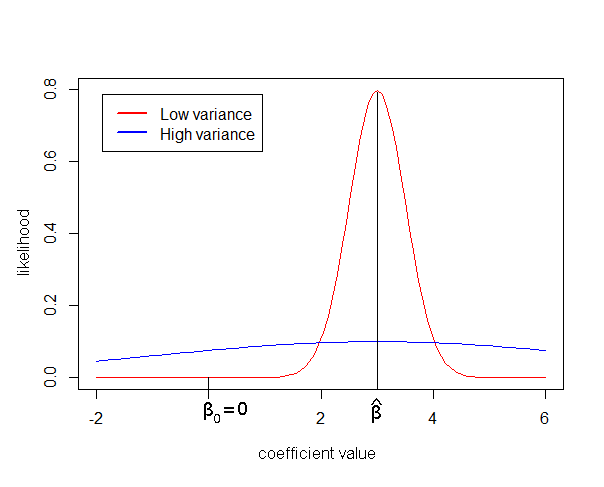
\includegraphics[scale=.7]{images/wald_test}
	\caption{Voorbeeld Wald test variantie visualisatie. Beide curves geven dezelfde maximum likelihood schatting voor $\hat{\beta}$. De rode curve heeft echter een lage variantie, wat veel evidentie biedt om de null-hypothese te verwerpen. De blauwe curve heeft een hoge variantie, in dit geval is het niet meteen duidelijk dat $\hat{\beta}$ echt verschilt van $\beta_{0}$ en dus kunnen we de null-hypothese niet verwerpen.}
	\label{fig:D:evaluation-wald-test}
\end{figure}

\subsection{Resultaten}
Tabel \ref{tab:D:evaluation-case2-dimensions} geeft een overzicht van de dimensies van de gebruikte datasets. De resultaten van de significantietests voor alle modellen worden getoond in de tabellen \ref{tab:D:evaluation-surv-individual} en \ref{tab:D:evaluation-surv-integrated}. Het is meteen duidelijk dat bijna alle modellen niet significant zijn. De berekende p-waarden zijn duidelijk ver boven de vooropgestelde grens van 0.05. Dat terzijde is het interessant om op te merken dat alle ge\"integreerde modellen duidelijk meer significant zijn dan de modellen voor individuele datasets. Meer nog, het partieel ge\"integreerde model is het enige model dat het significantie niveau van 0.05 bereikt. Er zou echter meer onderzoek moeten gebeuren om de werkelijke predictieve waarde van dit model te onderzoeken, maar voor deze studie is het duidelijk dat dit model het beste model is. En dus kunnen we concluderen dat de ge\"integreerde modellen ook hier aantonen dat ze een positieve impact hebben op de performantie van de bekomen modellen.
\begin{table}
	\centering
	\begin{tabular}{lcc}
		\toprule
		Dataset naam & Aantal variabelen & Aantal pati\"enten \\
		\midrule
		Copy Number Variations & 16 & 219\\
		messenger RNA & 3869 & 219 \\
		micro RNA & 414 & 219 \\
		\bottomrule
	\end{tabular}
	\caption{Dimensies voor de datasets die gebruikt werden in de overlevingsanalyse.}
	\label{tab:D:evaluation-case2-dimensions}
\end{table}

\begin{table}
	\centering
	\begin{tabular}{lccc}
		\toprule
		& CNV    & mRNA & miRNA \\
		\midrule
		Wald test 					& 0.17 & 0.13  & 1.46 \\
		P-waarde 					& 0.6799 & 0.7209  & 0.2276 \\
		\bottomrule
	\end{tabular}
	\caption{Significantie waarden voor de overlevingsmodellen voor individuele datasets}
	\label{tab:D:evaluation-surv-individual}
\end{table}

\begin{table}
	\centering
	\begin{tabular}{lccc} 
		\toprule
		& Early & Intermediate & Late\\
		\midrule
		Wald test 					& 2.43 & 3.89 & 1.98 \\
		P-waarde 					& 0.1192 & 0.0485 & 0.1595 \\
		\bottomrule
	\end{tabular}
	\caption{Significantie waarden voor de ge\"integreerde overlevingsmodellen}
	\label{tab:D:evaluation-surv-integrated}
\end{table}

\section{Conclusie}
\label{cha:D:conclusie}
Het eerste hoofdstuk toont aan dat er een nood is aan data-integratie methoden door de steeds groeiende datasets waarmee we moeten werken. Door op een slimme manier verschillende datasets te integreren kunnen we predictieve modellen bouwen die beter presteren. \\ \\
Vervolgens beschreven we wat predictieve modellen inhouden en we toonden twee concrete voorbeelden: logistieke regressie - en cox modellen.  \\ \\
Met deze informatie konden we vervolgens de verschillende integratie strategi\"en voorstellen. De eerste strategie, vroege integratie, voegt alle datasets aan elkaar door overeenkomende datapunten te linken. De tweede strategie, late integratie, bouwt individuele modellen voor elke dataset, ge\"inspireerd op het concept van ensemble-leren. De laatste strategie, parti\"ele integratie, bouwt het predictief model in twee stappen en maakt gebruik van de variabele selectie eigenschap in de lasso regularisatie. \\ \\
Om aan te tonen dat de verschillende integratie strategie\"en een impact hebben op de performantie van de predictieve modellen, passen we de strategie\"en toe in twee case studies met echte gegevens over kankerpati\"enten. De eerste studie gebruikt logistieke regressie modellen. De data voor deze studie komt van het Universitair Ziekenhuis te Leuven en betreft scan-gegevens voor pati\"enten met darmkanker. De resultaten van deze studie tonen een duidelijke verbetering van de performantie door het gebruik van integratie. De tweede case studie gebruikt cox proportionele risico modellen. De data van deze studie kwam van de online TCGA database. De resultaten in deze studie waren minder evindent, maar we kunnen toch besluiten dat ook in dit geval de ge\"integreerde modellen beter presteren dan de individuele modellen. En specifiek het partieel ge\"integreerde model bleek het beste te zijn. Beide studies leveren daarom evidentie aan dat integratie van datasets inderdaad de performantie ten goede komt, en dat verschillende strategie\"en een verschillende impact hebben. \\ \\
Het moet echter duidelijk zijn dat dit niet het einde van de studie is. In dit thesis toonden we drie verschillende integratie strategie\"en, maar er zijn duidelijk nog veel andere manier mogelijk om datasets te integreren. Verder spitste de case studies in dit geval zich toe op twee lineaire modellen: logistieke regressie- en cox modellen. Een interessante uitbreiding is om te kijken of deze claims ook gelden voor andere (niet-lineaire) methoden. \\ \\
Daarnaast moeten we in ons achterhoofd onthouden dat deze studie kadert in een grotere studie wiens doel het is om patronen en nieuwe inzichten te vinden in de grote hoeveelheden kankergegevens waarover we beschikken. Door betere predictieve modellen te bouwen kunnen we in de toekomst nieuwe inzichten verkrijgen in de manier waarop kankers ontstaan en zich ontwikkelen. Dit zal op zijn beurt in de toekomst een weg bieden naar nieuwe behandelingen voor kanker.


\end{abstract*}

%%% Local Variables: 
%%% mode: latex
%%% TeX-master: "thesis"
%%% End: 
